\documentclass[11pt,a4paper]{article}

\usepackage[margin=1in]{geometry}
\usepackage[utf8]{inputenc}
\usepackage[T1]{fontenc}
\usepackage{lmodern}
\usepackage{microtype}
\usepackage{amsmath}
\usepackage{amsfonts}
\usepackage{amssymb}
\usepackage{booktabs}
\usepackage{nicefrac}
\usepackage{xcolor}
\usepackage{hyperref}
\usepackage{url}
\usepackage[numbers,compress]{natbib}
\usepackage{listings}
\usepackage{tikz}
\usetikzlibrary{fit}
\usepackage{pgfplots}
\pgfplotsset{compat=1.18}

\hypersetup{
  colorlinks=true,
  linkcolor=blue!70!black,
  citecolor=blue!70!black,
  urlcolor=blue!70!black,
}

\lstset{
  basicstyle=\ttfamily\small,
  breaklines=true,
  frame=single,
  rulecolor=\color{gray!40},
  backgroundcolor=\color{gray!5},
}

\title{\textbf{Emerge: A Muscle-Memory Flywheel for\\[4pt]
       Crystallizing AI Agent Execution Patterns}}

\author{
  Zao Zhang \\[2pt]
  School of Electronic and Information Engineering \\
  Beihang University, Beijing 100191, China \\[2pt]
  \texttt{zzchun12826@buaa.edu.cn}
}

\date{April 2025}

\begin{document}

\maketitle
\thispagestyle{empty}

\begin{abstract}
AI agents today pay full inference cost on every invocation---even for tasks performed identically hundreds
of times before.
We propose \emph{policy-driven crystallization}: a mechanism by which repeated agent actions are tracked by
semantic intent, promoted through a three-stage reliability lifecycle
(\textsc{explore} $\to$ \textsc{canary} $\to$ \textsc{stable}), and ultimately \emph{crystallized} into
deterministic, verifiable pipelines that execute with zero LLM overhead.
We instantiate this idea in \textbf{Emerge}, a Claude Code plugin, and introduce two complementary flywheels:
a \emph{forward flywheel} that crystallizes AI reasoning into code,
and an \emph{Operator Intelligence Loop}---a reverse flywheel that observes human operators,
detects high-frequency behavioral patterns, and hands them off to the AI layer.
As both flywheels accumulate stable patterns, the system converges toward a state where neither the AI
nor the human needs to perform mechanical, repetitive work:
reasoning is replaced by pipelines, and human execution is replaced by learned automation.
We present the design, the policy framework with its formal promotion thresholds,
and the architectural invariant that keeps all policy state local while delegating execution to
arbitrary remote environments.
\end{abstract}

% ─────────────────────────────────────────────
\section{Introduction}
% ─────────────────────────────────────────────

Large language model (LLM) agents are increasingly deployed for domain-specific automation:
querying CAD models, applying parametric changes, verifying structural constraints, and logging outcomes.
Each of these tasks, when performed through ad-hoc LLM reasoning, incurs the full cost of model inference---even
when the task is semantically identical to one performed hundreds of times before.

Humans address this through \emph{muscle memory}: with enough repetition, a skilled operator stops deliberating
and acts reflexively. The cognitive overhead is amortized until it approaches zero.
Can AI agents develop an analogous property?

Emerge answers this with a \emph{muscle-memory flywheel}---a feedback system that:
\begin{enumerate}
  \item tracks every agent tool call by semantic intent;
  \item accumulates evidence of reliability through a formal policy lifecycle;
  \item crystallizes reliable patterns into deterministic, verifiable pipelines; and
  \item short-circuits future invocations through a flywheel bridge once patterns are trusted.
\end{enumerate}

Our contributions are:
\begin{itemize}
  \item A \textbf{policy lifecycle framework} (\textsc{explore} $\to$ \textsc{canary} $\to$ \textsc{stable})
        with configurable thresholds grounded in success rate, verification rate, and human-fix rate.
  \item A \textbf{flywheel bridge} mechanism for zero-overhead execution of stable patterns.
  \item A \textbf{two-channel execution architecture} separating policy state (always local)
        from execution (optionally delegated to a remote runner).
  \item An \textbf{Operator Intelligence Loop}: a reverse flywheel that crystallizes human operator
        patterns, not just AI patterns.
\end{itemize}

% ─────────────────────────────────────────────
\section{Background and Motivation}
% ─────────────────────────────────────────────

\subsection{The Cost of Repeated Reasoning}

Current agent frameworks~\cite{yao2022react,significant2023autogpt,langchain2022} treat every invocation
as independent.
A \texttt{read\_cad\_state} call at step~1 and an identical call at step~100 incur the same inference cost.
For agents operating in tight loops---reading sensor state, issuing corrections, verifying outcomes---this is
significant and unnecessary overhead.

Semantic caching~\cite{bang2023gptcache} partially addresses this for identical inputs but does not generalize
across semantically equivalent invocations with different parameters, nor does it support structured output
contracts with verification.

\subsection{Program Synthesis from Execution Traces}

Program synthesis~\cite{ellis2021dreamcoder,gulwani2017program} converts natural-language specifications into
executable code.
Emerge takes a related but distinct approach: rather than generating programs from specifications, it
\emph{extracts} programs from observed agent behavior.
The write-ahead log (WAL) records every successful execution path; crystallization distills these into a
stable, verifiable pipeline.
This is closer in spirit to inductive programming~\cite{de2008inductive} but operates continuously over live
agent sessions rather than in a single batch pass.

\subsection{Canary Deployment as a Reliability Primitive}

Canary deployment gradually shifts traffic to new software versions while monitoring for regressions,
limiting the blast radius of changes that appear reliable in staging but degrade in production.
We adapt this pattern to AI-generated execution candidates: a candidate enters canary rollout at 20\%
volume before earning full trust at stable (100\%).
To our knowledge, this is the first application of canary rollout semantics to AI agent execution patterns.

% ─────────────────────────────────────────────
\section{System Design}
% ─────────────────────────────────────────────

\subsection{Architecture}

Emerge runs as a single stdio MCP server inside the Claude Code process.
The daemon (\texttt{EmergeDaemon}) is the sole control plane: it routes all tool calls, maintains policy
state, and owns the WAL.
Heavy or GUI-dependent execution is delegated to an optional HTTP remote runner, while all policy state,
registry, and WAL remain local.
Figure~\ref{fig:arch} summarizes the component layout.

\begin{figure}[h]
\centering
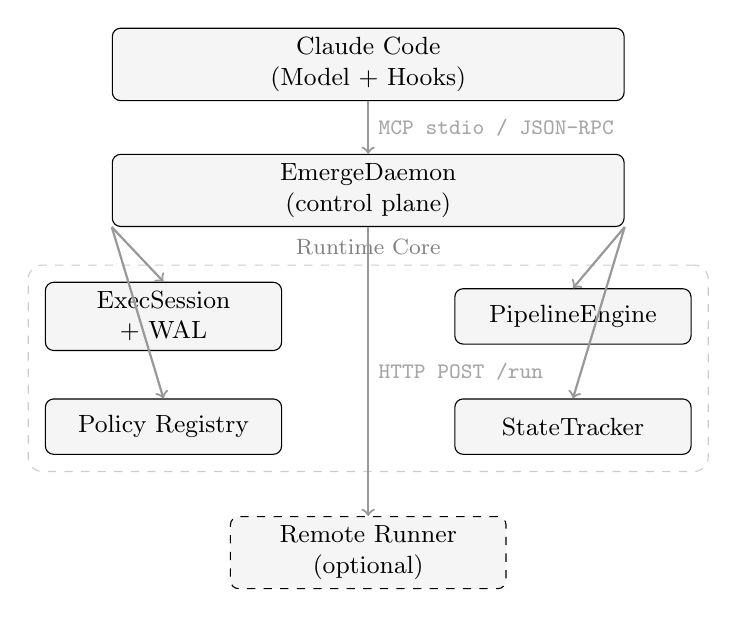
\begin{tikzpicture}[
  box/.style={draw, rounded corners=3pt, fill=gray!8, minimum height=2em,
              minimum width=3.0cm, align=center, font=\small},
  top/.style={box, minimum width=6.5cm},
  opt/.style={box, minimum width=3.5cm, dashed},
  arr/.style={->, thick, color=gray!80},
  lbl/.style={font=\footnotesize\ttfamily, color=gray!70}
]
  % Top tier
  \node[top] (cc) at (0, 4.2) {Claude Code\\(Model + Hooks)};
  \node[top] (d)  at (0, 2.6) {EmergeDaemon\\(control plane)};

  % Runtime core — 2×2 grid, no overlap
  \node[box] (es) at (-2.6, 1.0) {ExecSession\\+ WAL};
  \node[box] (pe) at ( 2.6, 1.0) {PipelineEngine};
  \node[box] (pr) at (-2.6,-0.4) {Policy Registry};
  \node[box] (st) at ( 2.6,-0.4) {StateTracker};

  % Runtime core bounding box
  \node[draw=gray!40, dashed, rounded corners=5pt,
        fit=(es)(pe)(pr)(st), inner sep=6pt,
        label={[font=\footnotesize\color{gray}]above:Runtime Core}] {};

  % Remote runner
  \node[opt] (rr) at (0,-2.0) {Remote Runner\\(optional)};

  % Edges
  \draw[arr] (cc) -- node[right, lbl]{MCP stdio / JSON-RPC} (d);
  \draw[arr] (d.south west) -- (es.north);
  \draw[arr] (d.south east) -- (pe.north);
  \draw[arr] (d.south west) -- (pr.north);
  \draw[arr] (d.south east) -- (st.north);
  \draw[arr] (d)  -- node[right, lbl]{HTTP POST /run} (rr);
\end{tikzpicture}
\caption{Emerge component layout. The daemon is the single control plane; the remote runner is a
         stateless executor that never touches policy state.}
\label{fig:arch}
\end{figure}

A key architectural invariant: \textbf{policy never leaves the daemon}.
Remote runners receive self-contained \texttt{icc\_exec} payloads and return stdout JSON.
Connector files never need to exist on the runner machine; switching execution hosts is a URL change only.

\subsection{The \texttt{icc\_*} Tool Surface}

Emerge exposes five MCP tools (Table~\ref{tab:tools}).

\begin{table}[h]
\centering
\caption{Emerge MCP tools.}
\label{tab:tools}
\begin{tabular}{@{}lp{9cm}@{}}
\toprule
\textbf{Tool} & \textbf{Role} \\
\midrule
\texttt{icc\_exec}        & Execute Python in a persistent local session. Tracks \texttt{intent\_signature} for the flywheel. Optionally routes to a remote runner. \\
\texttt{icc\_read}        & Run a deterministic read pipeline (local or remote). Returns structured rows with verification state. Falls back to a \texttt{pipeline\_missing} hint when no pipeline exists yet. \\
\texttt{icc\_write}       & Run a deterministic write pipeline with rollback/stop policy enforcement. \\
\texttt{icc\_crystallize} & Generate \texttt{.py} + \texttt{.yaml} pipeline files from WAL history for a given \texttt{intent\_signature}. Always writes locally. \\
\texttt{icc\_reconcile}   & Record a human correction. Increments \texttt{human\_fix\_rate} on the most-recently-used matching candidate. \\
\bottomrule
\end{tabular}
\end{table}

\subsection{Policy Lifecycle}
\label{sec:lifecycle}

Each distinct \texttt{intent\_signature} accumulates a \emph{candidate}---a record of execution attempts,
successes, verification results, and human corrections.
The policy engine evaluates candidates against configurable thresholds:

\begin{equation}
  \textsc{explore} \xrightarrow{A \geq 20,\; S \geq 0.95,\; f \leq 0.05}
  \textsc{canary} \xrightarrow{A \geq 40,\; S \geq 0.97,\; V \geq 0.99}
  \textsc{stable}
  \label{eq:lifecycle}
\end{equation}

\noindent where $A$ = attempt count, $S$ = success rate, $V$ = verify rate, $f$ = human-fix rate.
Any stage demotes to \textsc{explore} on two consecutive failures or a window success rate below 90\%.

The \textsc{canary} stage is critical: it allows a pattern to run in partial production volume before full
promotion, catching cases where high exploration success rate does not generalize.

\subsection{Flywheel Bridge}

When a candidate reaches \textsc{stable}, subsequent \texttt{icc\_exec} calls with matching
\texttt{intent\_signature} and \texttt{script\_ref} are intercepted \emph{before} model inference.
The daemon resolves the stable pipeline and returns its result directly.
We call this the \emph{flywheel bridge}: the pattern has been internalized and no longer requires reasoning.

Bridge keys follow the canonical form:
\begin{lstlisting}
flywheel::<pipeline_id>::<intent_signature>::<script_ref>
\end{lstlisting}

If the pipeline fails or the candidate demotes, the bridge disables transparently and the call falls back to
normal exec. This makes promotion and demotion seamless from the agent's perspective.

\subsection{Remote Execution Architecture}
\label{sec:remote}

For workloads requiring specific hardware, GUI access, or OS-native tooling (e.g.\ AutoCAD COM objects on a
Windows VM), Emerge routes \texttt{icc\_exec} calls to a remote HTTP runner via \texttt{RunnerRouter}.

\texttt{icc\_read} and \texttt{icc\_write} are \emph{not} forwarded to the runner as pipeline calls.
Instead, the daemon loads the pipeline \texttt{.py} + \texttt{.yaml} locally, builds a self-contained inline
code payload (stripping \texttt{from \_\_future\_\_} imports that are invalid inside \texttt{exec()}),
and sends it as \texttt{icc\_exec}.
This preserves three properties:

\begin{enumerate}
  \item \textbf{Portability}: no connector files on runner; connector updates deploy immediately without runner redeploy.
  \item \textbf{Policy locality}: all lifecycle transitions happen in the daemon regardless of execution target.
  \item \textbf{Isolation}: runners execute opaque code payloads and never access policy state or registry.
\end{enumerate}

\subsection{ExecSession and WAL}

Each \texttt{target\_profile} has an independent \texttt{ExecSession}---a durable Python namespace that
persists across tool calls within a session.
Successful executions are appended to a write-ahead log (\texttt{wal.jsonl}).
On restart, the WAL is replayed to reconstruct session state, excluding calls marked \texttt{no\_replay=True}
(external side effects such as COM calls or file writes).

The WAL is the primary input to \texttt{icc\_crystallize}: the crystallizer selects high-quality execution
traces matching the target \texttt{intent\_signature} and synthesizes a \texttt{run\_read} or
\texttt{run\_write} function body from them.

% ─────────────────────────────────────────────
\section{Operator Intelligence Loop}
% ─────────────────────────────────────────────

The flywheel described in Section~\ref{sec:lifecycle} crystallizes \emph{AI} execution patterns.
We propose an extension---the \textbf{Operator Intelligence Loop}---that applies the same principle to
\emph{human} operators.

\subsection{Motivation}

In human-in-the-loop deployments, operators perform repetitive sequences: reviewing AI output, clicking
approve, checking logs, adjusting parameters.
These patterns are as amenable to crystallization as AI exec patterns, yet current tooling treats every
operator action as independent.
The Operator Intelligence Loop closes this gap.

\subsection{Design}

The loop consists of three components:

\textbf{Monitor.}
A background process observes operator behavior---tool invocations, UI interactions, clipboard patterns---and
logs structured events with semantic annotations and timestamps.

\textbf{Auditor.}
On a configurable time window (default: 5~minutes), the auditor detects high-frequency patterns and surfaces
a native GUI popup:
\begin{quote}
  \emph{``You've performed \texttt{verify-then-approve-layer-count} 8 times today. Want me to take this?''}
\end{quote}
The operator can accept, reject, or defer.

\textbf{Distiller.}
On acceptance, the operator's action sequence is extracted, an \texttt{intent\_signature} is assigned,
and the pattern enters the same \textsc{explore} $\to$ \textsc{canary} $\to$ \textsc{stable} lifecycle
as AI-generated patterns.

\subsection{The Convergence Property}

Both flywheels---AI action crystallization and operator pattern crystallization---converge to the same
artifact: entries in the pipeline registry.
The distinction is only the \emph{source of evidence}.
Over time, the registry accumulates patterns from both human and AI sources,
and the system becomes increasingly capable of autonomous execution across both axes.
Figure~\ref{fig:convergence} illustrates this duality.

\begin{figure}[h]
\centering
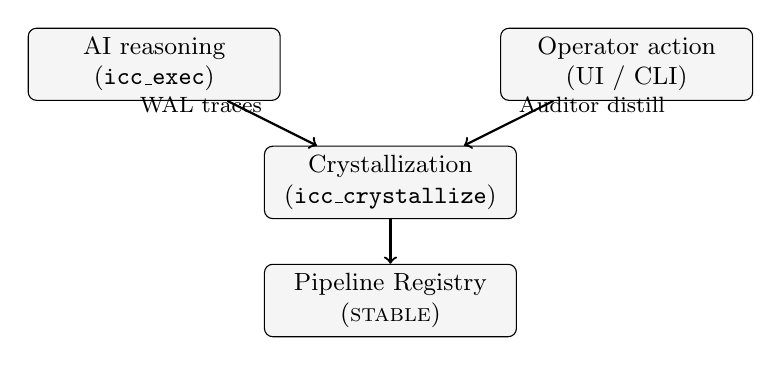
\begin{tikzpicture}[
  box/.style={draw, rounded corners=3pt, fill=gray!8, minimum height=1.8em, align=center, font=\small},
  arr/.style={->, thick}
]
  \node[box, minimum width=3.2cm] (ai)  at (-3, 1.5) {AI reasoning\\(\texttt{icc\_exec})};
  \node[box, minimum width=3.2cm] (op)  at ( 3, 1.5) {Operator action\\(UI / CLI)};
  \node[box, minimum width=3.2cm] (cr)  at ( 0, 0)   {Crystallization\\(\texttt{icc\_crystallize})};
  \node[box, minimum width=3.2cm] (reg) at ( 0,-1.5)  {Pipeline Registry\\(\textsc{stable})};

  \draw[arr] (ai) -- node[above left, font=\footnotesize]{WAL traces} (cr);
  \draw[arr] (op) -- node[above right, font=\footnotesize]{Auditor distill} (cr);
  \draw[arr] (cr) -- (reg);
\end{tikzpicture}
\caption{Both AI and operator patterns converge to the same pipeline registry.}
\label{fig:convergence}
\end{figure}

% ─────────────────────────────────────────────
\section{Implementation}
% ─────────────────────────────────────────────

Emerge is implemented in Python~3.11+ as a Claude Code plugin.
Key implementation decisions:

\paragraph{Policy storage.}
Two files: \texttt{candidates.json} (per-session, per-\texttt{intent\_signature} counters)
and \texttt{pipelines-registry.json} (global, per-pipeline lifecycle state).
All writes are atomic (temp file + rename) to prevent corruption under concurrent access.

\paragraph{Human-fix targeting.}
\texttt{icc\_reconcile} must increment \texttt{human\_fix\_rate} on the \emph{correct} candidate
when multiple candidates share the same \texttt{intent\_signature}.
We select by \texttt{last\_ts\_ms}---the candidate most recently used is the one active at correction time.
This prevents corrections from inflating rates on dormant candidates.

\paragraph{\texttt{from \_\_future\_\_} stripping.}
Pipeline \texttt{.py} files may contain \texttt{from \_\_future\_\_ import annotations}.
Since pipelines are executed via \texttt{exec()} inside the remote runner,
these imports are stripped before injection---they raise \texttt{SyntaxError} when appearing
non-first inside an \texttt{exec()} string.

\paragraph{Test suite.}
134 passing tests covering unit, integration, and MCP tool paths including flywheel bridge,
remote pipeline execution, and policy lifecycle transitions.
The integration suite exercises the full \texttt{EmergeDaemon.call\_tool()} stack against real
in-process sessions rather than mocks.

% ─────────────────────────────────────────────
\section{Related Work}
% ─────────────────────────────────────────────

\paragraph{LLM agent frameworks.}
ReAct~\cite{yao2022react}, AutoGPT~\cite{significant2023autogpt}, and LangChain~\cite{langchain2022}
provide general agent scaffolding but treat each invocation independently without policy-driven acceleration.

\paragraph{Semantic caching.}
GPTCache~\cite{bang2023gptcache} and similar systems cache LLM outputs for repeated queries.
Emerge differs in that crystallized pipelines produce new structured outputs (not cached prior outputs)
and enforce verification contracts.

\paragraph{Program synthesis.}
DreamCoder~\cite{ellis2021dreamcoder} and related systems~\cite{gulwani2017program} learn reusable program
abstractions.
Emerge performs continuous online synthesis from live execution traces rather than offline batch synthesis,
and targets operational reliability (canary/stable thresholds) rather than expressiveness.

\paragraph{Canary deployment.}
Canary releases are standard practice in large-scale software delivery~\cite{humble2010continuous},
gradually shifting traffic to new versions while monitoring for regressions.
We apply the same rollout semantics to AI-generated execution patterns---to our knowledge the first such application.

\paragraph{Human-in-the-loop and interactive teaching.}
Interactive machine teaching~\cite{simard2017imt} uses human signals to correct model behavior.
The Operator Intelligence Loop instead treats human behavioral \emph{patterns} as automation targets,
not model corrections---a complementary but distinct use of human signal.

% ─────────────────────────────────────────────
\section{Discussion and Limitations}
% ─────────────────────────────────────────────

\paragraph{Threshold sensitivity.}
The default thresholds ($A \geq 20$, $S \geq 0.95$, etc.) are empirically motivated but not formally derived.
Different domains may require different calibration; all thresholds are exposed as configurable via
\texttt{\textasciitilde/.emerge/settings.json}.

\paragraph{Crystallization quality.}
The quality of synthesized pipelines depends on WAL trace quality.
Noisy or highly variable exec sessions may produce pipelines that pass canary under favorable conditions
but fail under distribution shift.
The \texttt{human\_fix\_rate} signal provides a feedback mechanism but does not replace human review of
crystallized code.

\paragraph{Operator privacy.}
The Operator Intelligence Loop observes operator behavior, which raises privacy considerations in multi-user
deployments.
A production implementation must enforce local-only storage and explicit per-operator opt-in.

\paragraph{Scope.}
Emerge is currently evaluated within the Claude Code plugin ecosystem.
The core design---policy lifecycle, flywheel bridge, two-channel execution---is architecture-agnostic and
applicable to any agent system that performs repeated structured work.

% ─────────────────────────────────────────────
\section{Conclusion}
% ─────────────────────────────────────────────

We presented Emerge, a muscle-memory flywheel for AI agents.
The policy lifecycle (\textsc{explore} $\to$ \textsc{canary} $\to$ \textsc{stable}) provides a principled
path from exploration to trust.
The flywheel bridge eliminates inference overhead for stable patterns.
The two-channel architecture keeps policy local while supporting arbitrary remote execution targets.
The Operator Intelligence Loop extends crystallization to human behavior, progressively automating the
mechanical components of operator work.

The pattern of \emph{policy-driven crystallization}---tracking, validating, and internalizing execution
patterns through staged promotion---we believe generalizes beyond any single agent platform to any system
that performs repeated structured work.

% ─────────────────────────────────────────────
\bibliographystyle{abbrvnat}
\begin{thebibliography}{99}

\bibitem{yao2022react}
S. Yao, J. Zhao, D. Yu, N. Du, I. Shafran, K. Narasimhan, and Y. Cao.
\newblock {ReAct}: Synergizing Reasoning and Acting in Language Models.
\newblock In \emph{ICLR}, 2023.

\bibitem{significant2023autogpt}
Significant Gravitas.
\newblock {Auto-GPT}: An Autonomous {GPT-4} Experiment.
\newblock \url{https://github.com/Significant-Gravitas/AutoGPT}, 2023.

\bibitem{langchain2022}
H. Chase.
\newblock {LangChain}.
\newblock \url{https://github.com/langchain-ai/langchain}, 2022.

\bibitem{bang2023gptcache}
F. Bang.
\newblock {GPTCache}: An Open-Source Semantic Cache for {LLM} Applications Enabling Faster Answers and Cost Savings.
\newblock In \emph{Proc.\ 3rd Workshop for NLP Open Source Software (NLP-OSS)}, pp.\ 212--218. ACL, 2023.

\bibitem{ellis2021dreamcoder}
K. Ellis, C. Wong, M. Nye, M. Sable-Meyer, L. Morales, L. Hewitt, L. Cary, A. Solar-Lezama, and J. B. Tenenbaum.
\newblock {DreamCoder}: Bootstrapping Inductive Program Synthesis with Wake-Sleep Library Learning.
\newblock In \emph{PLDI}, 2021.

\bibitem{gulwani2017program}
S. Gulwani, O. Polozov, and R. Singh.
\newblock Program Synthesis.
\newblock \emph{Foundations and Trends in Programming Languages}, 4(1-2):1--119, 2017.

\bibitem{de2008inductive}
L. De Raedt.
\newblock \emph{Logical and Relational Learning}.
\newblock Springer, 2008.

\bibitem{humble2010continuous}
J. Humble and D. Farley.
\newblock \emph{Continuous Delivery: Reliable Software Releases through Build, Test, and Deployment Automation}.
\newblock Addison-Wesley, 2010.

\bibitem{simard2017imt}
P. Y. Simard, S. Amershi, D. M. Chickering, A. E. Pelton, S. Ghorashi, C. Meek, G. Ramos, J. Suh,
J. Verwey, M. Wang, and J. Wernsing.
\newblock Machine Teaching: A New Paradigm for Building Machine Learning Systems.
\newblock \emph{arXiv:1707.06742}, 2017.

\end{thebibliography}

\end{document}
